\documentclass{beamer}

\usepackage[utf8]{inputenc}
\usepackage[T1]{fontenc}

%\usepackage[backend=biber]{biblatex}
%\addbibresource{biblio.bib}
\usepackage[T1]{fontenc}
\usepackage[boxed,linesnumbered,noend]{algorithm2e}
\usepackage{listings}
\usepackage{xcolor}


\usetheme{ENSLyon}
\title[MPNA]{Performance evaluation: Arnoldi's algorithm}
\author[N.D.]{Nicolas Derumigny}
\institute[]{ENS Lyon}
\date{29 Novembre 2017}
  \setbeamersize{text margin left=10mm}
  \setbeamersize{text margin right=10mm}

\setbeamertemplate{navigation symbols}{}
\usecolortheme{ENSLyon_blue}


\definecolor{mGreen}{rgb}{0,0.6,0}
\definecolor{mGray}{rgb}{0.5,0.5,0.5}
\definecolor{mPurple}{rgb}{0.58,0,0.82}
\definecolor{backgroundColour}{rgb}{0.95,0.95,0.92}

\lstset{
    language=C,
    backgroundcolor=\color{backgroundColour}, 
    basicstyle=\footnotesize\ttfamily\color{black},
    keywordstyle=\bfseries\color{teal},
    commentstyle=\color{mGreen},
    stringstyle=\color{blue}
}
\begin{document}
\begin{frame}
	\titlepage
	\begin{center}
	
\includegraphics[height=0.5cm]{logoens.pdf}

	\end{center}
\end{frame}

\section{Algorithm}
\begin{frame}
\begin{algorithm}[H]
$q_1 = \dfrac{q}{||q||}$ \\
\For{k=1 à m-1}{
	$w=Aq_k$\\
	\For{j=1 à k}{
		$h_{j,k}=\langle w,q_0 \rangle$\\
		$w=w-h_{j,k}\cdot q_j$
	}
	$h_{k+1, k}=||w||_2$\\
	$q_{k+1}=\dfrac{w}{h_{k+1,k}}$
}
\caption{Arnoldi's algorithm}
\end{algorithm}
\end{frame}

\section{Time measurements}
\begin{frame}[fragile]{How to measure the execution time?}
\begin{itemize}
\item Use \texttt{time.h}
\end{itemize}
\bigskip
\begin{lstlisting}[frame=single]
#include <time.h>

int main(){
	clock_t start, end;
	start = clock();
	//program here
	end = clock();
	printf("%f\n", (end-start)/CLOCKS_PER_SEC));
}
\end{lstlisting}
\end{frame}

\begin{frame}{Complexity}
\begin{itemize}
\item {Time:} The matrix-vector product dominates $\Rightarrow$ $O(n^2)$
\bigskip
\item {Space:} The storage of $A$ dominates $\Rightarrow$ $O(n^2)$
\end{itemize}
\end{frame}

\section{Results}
\begin{frame}{i5-2520M}
\begin{columns}
\begin{column}{0.3\linewidth}
\begin{itemize}
\item Sandy Bridge
\end{itemize}
\end{column}
\begin{column}{0.3\linewidth}
\begin{itemize}
\item 3.5 GHz
\end{itemize}
\end{column}
\begin{column}{0.3\linewidth}
\begin{itemize}
\item Hyperthreaded Dual-core
\end{itemize}
\end{column}
\end{columns}
\begin{figure}
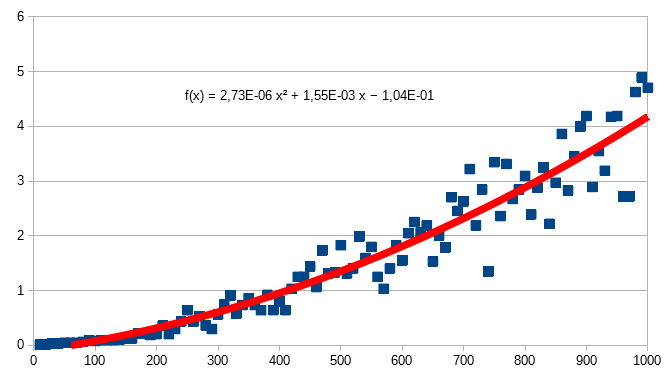
\includegraphics[width=0.82\linewidth]{lenovo-i5-2emeGen.png}
\caption{Performance evaluation on the i5-2520M}
\end{figure}
\end{frame}

%\begin{frame}{i5-6600k}
%\begin{columns}
%\begin{column}{0.3\linewidth}
%\begin{itemize}
%\item Skylake
%\end{itemize}
%\end{column}
%\begin{column}{0.3\linewidth}
%\begin{itemize}
%\item 3.9 GHz
%\end{itemize}
%\end{column}
%\begin{column}{0.3\linewidth}
%\begin{itemize}
%\item Quad-core
%\end{itemize}
%\end{column}
%\end{columns}
%\begin{figure}
%\includegraphics[width=0.82\linewidth]{i5-6600K.png}
%\caption{Performance evaluation on the i5-6600K}
%\end{figure}
%\end{frame}
%\begin{frame}{Bibliographie}
%\nocite{*}
%\printbibliography    
%\end{frame}

\end{document}
